\documentclass[11pt]{article}
\usepackage[utf8]{inputenc}

% Increase main memory size
\usepackage{etex}
\usepackage{morewrites}
\usepackage{multicol}
\usepackage{pgfplots}
\usepackage{tikz}
\usetikzlibrary{external}
\tikzexternalize[prefix=cached_models/]
% Ensure the directory exists
\immediate\write18{mkdir -p cached_models}

\usepackage{etex}
\usepackage{morewrites}
\usepackage{enumitem}
\usepackage{float}

\listfiles

\usepackage{amsmath, amssymb, amsthm}
\usepackage{graphicx}
\usepackage{geometry}
\usepackage{array}
\usepackage{booktabs}
\usepackage{float}
\usepackage{verbatim}
\usetikzlibrary{3d}

% Page Layout
\geometry{a4paper, margin=1in}
\setlength\parindent{0pt}
\pgfplotsset{compat=1.18}

\title{\textbf{Principles of Math. Analysis: Self-Evaluation 1}}
\author{Nuño Cambero García}
\date{20-10-2025}

\begin{document}

\maketitle

\section*{Problem 1}
\begin{enumerate} [label = \alph*)]
    \item \textbf{\large Given the space \(X = \{1, 2, 3, 4, 5\}\), build the \(\sigma\)-algebra generated by the collection of sets:
        \[\mathcal{E} = \{\{1\}, \{1, 2\}, \{1, 5\}\}.\]}
        To build the \(\sigma\)-algebra generated by \(\mathcal{E}\), we need to include all possible unions, intersections, and complements of the sets in \(\mathcal{E}\). The generated \(\sigma\)-algebra will include:
        \begin{itemize}
            \item The empty set: \(\emptyset\), and the whole set: \(X = \{1, 2, 3, 4, 5\}\)
            \item The sets in \(\mathcal{E}\): \(\{1\}, \{1, 2\}, \{1, 5\}\), and its complements: \(\{2, 3, 4, 5\}, \{3, 4, 5\}, \{2, 3, 4\}\)
            \item Unions of the sets in \(\mathcal{E}\): \(\{1, 2, 5\}\), and the complement \(\{3, 4\}\)
        \end{itemize}
        After considering all combinations, the \(\sigma\)-algebra generated by \(\mathcal{E}\) is:
        \[\sigma (\mathcal{E}) = \{\emptyset, \{1\}, \{1, 2\}, \{1, 5\}, \{1, 2, 5\}, \{3, 4\}, \{2, 3, 4, 5\}, \{3, 4, 5\}, \{2, 3, 4\}, X\}.\]
    \item \textbf{\large Study if the function \(f : X \to \mathbb{R}\) defined by \(f(x) = x\) is measurable.}

        To determine if the function \(f\) is measurable, we need to check if the preimage of every Borel set in \(\mathbb{R}\) is in the \(\sigma\)-algebra generated by \(\mathcal{E}\). Let us try with \(\mathcal{B} = (-\infty, a]\) for various values of \(a\):
        \begin{itemize}
            \item For \(a < 1\): \(f^{-1}((-\infty, a]) = \emptyset \in \sigma(\mathcal{E})\)
            \item For \(1 \leq a < 2\): \(f^{-1}((-\infty, a]) = \{1\} \in \sigma(\mathcal{E})\)
            \item For \(2 \leq a < 3\): \(f^{-1}((-\infty, a]) = \{1, 2\} \in \sigma(\mathcal{E})\)
            \item For \(3 \leq a < 4\): \(f^{-1}((-\infty, a]) = \{1, 2, 3\} \notin \sigma(\mathcal{E})\)
        \end{itemize}
        Since there exists a Borel set (for example, \((-\infty, 4]\)) whose preimage is not in \(\sigma(\mathcal{E})\), the function \(f\) is not measurable.

        \begin{center}
            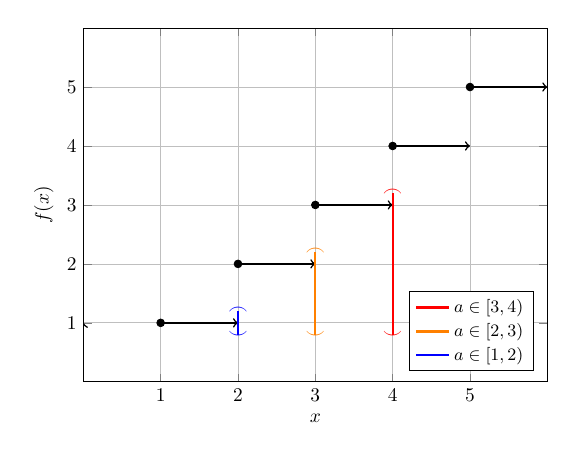
\begin{tikzpicture}[scale=0.7]
                \begin{axis}[
                    xlabel = \(x\),
                    ylabel = {\(f(x)\)},
                    xtick={1,2,3,4,5},
                    ytick={1,2,3,4,5},
                    grid=both,
                    ymin=0, ymax=6,
                    xmin=0, xmax=6,
                    width=10cm,
                    height=8cm,
                    legend pos=south east,
                    legend style={font=\small},
                ]

                \draw[->, thick] (0,0) -- (0,1);
                \draw[->, thick] (1,1) -- (2,1);
                \draw[->, thick] (2,2) -- (3,2);
                \draw[->, thick] (3,3) -- (4,3);
                \draw[->, thick] (4,4) -- (5,4);
                \draw[->, thick] (5,5) -- (6,5);


                \addplot[very thick, red] (4,0.8) node[]{$\smile$} -- (4,3.2) node[]{$\frown$};
                \addlegendentry{\(a \in [3, 4)\)}

                \addplot[very thick, orange] (3,0.8) node[]{$\smile$} -- (3,2.2) node[]{$\frown$};
                \addlegendentry{\(a \in [2, 3)\)}

                \addplot[very thick, blue] (2,0.8) node[]{$\smile$} -- (2,1.2) node[]{$\frown$};
                \addlegendentry{\(a \in [1, 2)\)}

                \addplot[only marks, mark=*, mark size=2pt] coordinates {
                    (1,1)
                    (2,2)
                    (3,3)
                    (4,4)
                    (5,5)
                };
                \end{axis}
            \end{tikzpicture}
        \end{center}
\end{enumerate}

\section*{Problem 2}
\textbf{\large Consider a mapping \(f : X \to Y\) where \((Y, \mathcal{A})\) is a measurable space and prove that
\[\mathcal{A}^{\prime} = \{f^{-1}(E) : E \in \mathcal{A}\}\]
is a \(\sigma\)-algebra in \(X\).}

To prove that \(\mathcal{A}^{\prime}\) is a \(\sigma\)-algebra in \(X\), we need to verify the three properties of a \(\sigma\)-algebra:
\begin{itemize}
    \item \textbf{Contains the empty set:} Since \(\emptyset \in \mathcal{A}\), we have \(f^{-1}(\emptyset) = \emptyset \in \mathcal{A}^{\prime}\).
    \item \textbf{Closed under complements:} If \(A \in \mathcal{A}^{\prime}\), then there exists \(E \in \mathcal{A}\) such that \(A = f^{-1}(E)\). The complement of \(A\) in \(X\) is:
    \[A^c = X \setminus A = X \setminus f^{-1}(E) = f^{-1}(Y \setminus E) = f^{-1}(E^c).\]
    Since \(E^c \in \mathcal{A}\), it follows that \(A^c \in \mathcal{A}^{\prime}\).
    \item \textbf{Closed under countable unions:} Let \(\{A_n\}_{n=1}^{\infty}\) be a sequence of sets in \(\mathcal{A}^{\prime}\). Then, for each \(n\), there exists \(E_n \in \mathcal{A}\) such that \(A_n = f^{-1}(E_n)\). The countable union of these sets is:
    \[\bigcup_{n=1}^{\infty} A_n = \bigcup_{n=1}^{\infty} f^{-1}(E_n) = f^{-1}\left(\bigcup_{n=1}^{\infty} E_n\right).\]
    Since \(\bigcup_{n=1}^{\infty} E_n \in \mathcal{A}\), it follows that \(\bigcup_{n=1}^{\infty} A_n \in \mathcal{A}^{\prime}\).
\end{itemize}
Since \(\mathcal{A}^{\prime}\) satisfies all three properties of a \(\sigma\)-algebra, we conclude that \(\mathcal{A}^{\prime}\) is indeed a \(\sigma\)-algebra in \(X\).

\section*{Problem 3}
\textbf{\large Use the definition to prove that if \((X, \mathcal{A}, \mu)\) is a measure space and the sets \(\{A_n\}_{n \in N}\) are in \(\mathcal{A}\) and satisfy:
\[A_1 \supseteq A_2 \supseteq A_3 \dots \supseteq A_n \supseteq \dots, \quad \text{with } \mu(A_1) < \infty,\]
then,
\[\mu (\bigcap_{n=1}^{\infty} A_n) = \lim_{n \to \infty} \mu(A_n).\]}

We can define a new sequence of sets \(B_n = A_1 \setminus A_n\). With \(A_n\) a decreasing sequence, \(B_n\) is an increasing sequence of sets and we have:
\[\bigcap_{n=1}^{\infty} A_n = A_1 \setminus \bigcup_{n=1}^{\infty} B_n.\]
By the properties of measures, we know that:
\[\mu\left(\bigcup_{n=1}^{\infty} B_n\right) = \lim_{n \to \infty} \mu(B_n).\]
Since \(B_n = A_1 \setminus A_n\), we have:
\[\mu(B_n) = \mu(A_1) - \mu(A_n).\]
Thus,
\[\mu\left(\bigcup_{n=1}^{\infty} B_n\right) = \lim_{n \to \infty} [\mu(A_1) - \mu(A_n)] = \mu(A_1) - \lim_{n \to \infty} \mu(A_n).\]
Now, substituting back into the expression for \(\mu\left(\bigcap_{n=1}^{\infty} A_n\right)\), we get:
\[\mu\left(\bigcap_{n=1}^{\infty} A_n\right) = \mu(A_1) - \mu\left(\bigcup_{n=1}^{\infty} B_n\right) = \mu(A_1) - [\mu(A_1) - \lim_{n \to \infty} \mu(A_n)] = \lim_{n \to \infty} \mu(A_n).\]

\section*{Problem 4}
\textbf{\large On the measurable space \((X, \mathcal{A})\), we consider two points \(x_0, x_1 \in X\) and define the function
\[\mu(A) = \begin{cases}
1, & \text{if } x_0 \in A \text{ or } x_1 \in A \text{ (only one of them)}, \\
2, & \text{if } x_0, x_1 \in A  \text{ (both)}, \\
0, & \text{if } x_0 \notin A \text{ and } x_1 \notin A.
\end{cases}\]
Prove that \(\mu\) is a measure on \(\mathcal{A}\).}

To prove that \(\mu\) is a measure on \(\mathcal{A}\), we need to verify the following properties:
\begin{itemize}
    \item \textbf{Non-negativity:} By definition, \(\mu(A) \geq 0\) for all \(A \in \mathcal{A}\).
    \item \textbf{Null empty set:} We have \(\mu(\emptyset) = 0\) since neither \(x_0\) nor \(x_1\) is in the empty set.
    \item \textbf{Countable additivity:} Let \(\{A_n\}_{n=1}^{\infty}\) be a sequence of disjoint sets in \(\mathcal{A}\). We need to show that:
    \[\mu\left(\bigcup_{n=1}^{\infty} A_n\right) = \sum_{n=1}^{\infty} \mu(A_n).\]
    We consider the following cases:
    \begin{itemize}
        \item If neither \(x_0\) nor \(x_1\) is in any of the \(A_n\), then \(\mu(A_n) = 0\) for all \(n\), and thus both sides equal 0.
        \item If exactly one of \(x_0\) or \(x_1\) is in one of the \(A_n\), say \(x_0 \in A_k\) for some \(k\), then \(\mu(A_k) = 1\) and \(\mu(A_n) = 0\) for all \(n \neq k\). Thus, the left side equals 1, and the right side also equals 1.
        \item If both \(x_0\) and \(x_1\) are in different \(A_n\), say \(x_0 \in A_k\) and \(x_1 \in A_m\) for \(k \neq m\), then \(\mu(A_k) = 1\) and \(\mu(A_m) = 1\), while \(\mu(A_n) = 0\) for all \(n \neq k, m\). Thus, the left side equals 2, and the right side also equals 2.
        \item If both \(x_0\) and \(x_1\) are in the same set \(A_k\), then \(\mu(A_k) = 2\) and \(\mu(A_n) = 0\) for all \(n \neq k\). Thus, the left side equals 2, and the right side also equals 2.
    \end{itemize}
\end{itemize}
Since all three properties are satisfied, we conclude that \(\mu\) is indeed a measure
\pagebreak
\section*{Problem 5}
\textbf{\large We consider the function:
\[g(x) = \arctan [x], \quad x \in \mathbb{R},\]
where \([x]\) is the integer part of \(x\).
\begin{enumerate} [label = \alph*)]
    \item Prove that \(g\) is a distribution function for some Lebesgue-Stieltjes measure \(\mu_g\).
    \item Obtain the measure of the following sets, approximating the infinite sets by an increasing sequence of sets:
        \[(0, 1), \quad [-1, 1], \quad A = \{x : |x^2 - 1| < 1\}, \quad (1, \infty), \quad \mathbb{R}.\]
\end{enumerate}}

For \(g\) to be a distribution function, it must be non-decreasing, right-continuous.
The function \(\arctan[x]\) is non-decreasing since \([x]\) is non-decreasing and \(\arctan\) is an increasing function. It is right-continuous because \([x]\) is right-continuous, and \(\arctan\) is continuous. 
Thus, \(g\) is a distribution function for some Lebesgue-Stieltjes measure \(\mu_g\).

To find the measure of the given sets, we use the properties of the Lebesgue-Stieltjes measure associated with \(g\):
\begin{itemize}
    \item For the interval \((0, 1)\):
    \[\mu_g((0, 1)) = g(1) - g(0) = \arctan(1) - \arctan(0) = \frac{\pi}{4} - 0 = \frac{\pi}{4}.\]
    \item For the interval \([-1, 1]\):
    \[\mu_g([-1, 1]) = g(1) - g(-1) = \arctan(1) - \arctan(-1) = \frac{\pi}{4} - \left(-\frac{\pi}{4}\right) = \frac{\pi}{2}.\]
    \item For the set \(A = \{x : |x^2 - 1| < 1\}\):
    This set can be rewritten as \((-\sqrt{2}, \sqrt{2}) \sim (-1, 1)\):
    \[\mu_g(A) = g(1) - g(-1) = \arctan(1) - \arctan(-1) = \frac{\pi}{4} - \left(-\frac{\pi}{4}\right) = \frac{\pi}{2}.\]
    \item For the interval \((1, \infty)\):
    \[\mu_g((1, \infty)) = \lim_{x \to \infty} g(x) - g(1) = \frac{\pi}{2} - \arctan(1) = \frac{\pi}{2} - \frac{\pi}{4} = \frac{\pi}{4}.\]
    \item For the entire real line \(\mathbb{R}\):
    \[\mu_g(\mathbb{R}) = \lim_{x \to \infty} g(x) - \lim_{x \to -\infty} g(x) = \frac{\pi}{2} - \left(-\frac{\pi}{2}\right) = \pi.\]
\end{itemize}

\end{document}